\documentclass[hyperref,french,usenames,xcolor=dvipsnames]{beamer}
 \mode<presentation>
{
\usepackage{beamerthemesplit}
\usetheme[compress,secheader]{Madrid}
%  \usecolortheme{orchid}
%	\setbeamercolor{alerted text}{fg=red!65!black}
  \setbeamercovered{transparent}
}
\usepackage{amsthm}
\usepackage{amsfonts}
\usepackage{amsmath}
\usepackage{graphicx}
%\usepackage{epsfig}
\usepackage{xspace}
\usepackage{stmaryrd}
%\usepackage{soul}
\usepackage[utf8]{inputenc}
%\usepackage[french]{algorithme}
%\usepackage[T1]{fontenc} %pour un beau PDF sous Linux ; à retirer sous Mac
\usepackage[french]{babel}

%\usepackage{ulem}
%\usepackage[english]{babel}
%\usepackage{times}
%\usepackage[utf8]{inputenc}
%\usepackage{amssymb}
%\usepackage{movie15}
%\usepackage{graphicx,color}
%\usepackage{hyperref}


%-----------------------------------------------------------

\definecolor{newcolor}{rgb}{0, 0, .90}
\definecolor{impcolor}{rgb}{.90, 0, 0}
\definecolor{darkergreen}{rgb}{0,0.5,0}
\definecolor{myorange}{rgb}{0.8,0.7,0}
\definecolor{myviolet}{rgb}{0.7,0.0,0.7}

\definecolor{lightpurple}{rgb}{0.83,0.27,1}
\definecolor{lightblue}{rgb}{0.27,0.9,0.9}



%\newcommand{\texthl}[1]{{\color{blue}#1}}
%\newcommand{\jaune}[1]{{\color{blue}#1}}
%\newcommand{\texthlb}[1]{{\color{orange}#1}}
%\newcommand{\orange}[1]{{\color{orange}#1}}
%\newcommand{\verte}[1]{{\color{green}#1}}
%\newcommand{\trad}{{\color{orange}{\bf $\leadsto$}}}

%\newcommand{\textcite}[1]{{\color{lightpurple}[#1]}}
%\newcommand{\textciten}[1]{{\color{lightpurple}#1}}

\newcommand{\texthl}[1]{{\color{red}#1}}
\newcommand{\jaune}[1]{{\color{red}#1}}
\newcommand{\texthlb}[1]{{\color{orange}#1}}
\newcommand{\orange}[1]{{\color{orange}#1}}
\newcommand{\verte}[1]{{\color{green}#1}}
\newcommand{\trad}{{\color{orange}{\bf $\leadsto$}}}

\newcommand{\textcite}[1]{{\color{myviolet}[#1]}}
\newcommand{\textciten}[1]{{\color{myviolet}#1}}

\newcommand{\montilde}{$\sim$}

\title[MarkUs]%
{Markus, an open-source web application to annotate student papers on-line}

%\subtitle{Applications aux réseaux de Petri temporels et aux automates
%  temporisés}

\author[MM, GM, NV, BV, KR, MC, SG]%
{\textbf{Morgan \textsc{Magnin}}, Guillaume \textsc{Moreau}, Nelle \textsc{Varoquaux}, Benjamin \textsc{Vialle}, Karen \textsc{Reid}, Mike \textsc{Conley} and Severin \textsc{Gehwolf}
}
\institute[ ]{
\structure{
École Centrale de Nantes / University of Toronto}
}

\date[07/03/2012]{ASME 2012 ESDA - 07/03/12}

%\date[] % (optional)
%{}

\subject{ASME 2012 11th Biennial Conference On Engineering Systems Design And Analysis}

\AtBeginSection[] % Do nothing for \section*
{
\frame<beamer>
	{
	\frametitle{Sommaire}
	\tableofcontents[current]
	}
}

\begin{document}

\frame{\titlepage}

% La proposition est d'axer la présentation du plus pédagogique au plus technique
% Faisant ainsi le lien avec la seconde présentation, orientée "technique"/"contribution"

\section*{Motivation}

%\subsection*{Motivation}

\frame
{
  \frametitle{Some challenging questions}

\begin{alertblock}{Motivation}
How to \textbf{efficiently} \textbf{manage} and \textbf{grade} students' papers (e.g. lab. works, projects, …)? \\
\begin{itemize}
        \item Submissions 
        \item Assessment  
        \item Feedback
        \item Distribution
        \item Record keeping
\end{itemize}
\end{alertblock}

\begin{alertblock}{Major issues}
\begin{itemize}
\item Huge \textbf{loads} of papers (~300-900 students per course) 
\item \textbf{Heterogeneity} of the teachers team
\item Digitalization 
\end{itemize}
\end{alertblock}
}

\frame
{
  \frametitle{Limits of the previous workflows}

\begin{alertblock}{Teachers' viewpoint:}
\begin{itemize}
\item \textbf{Loads} of students' submissions
\item Difficulty to \textbf{harmonize} assessment criteria between graders 
\item Paper lifecycle 
\begin{itemize}
\item Tons of papers that will never be assessed
\item When do you give the papers back to the students? 
\end{itemize}
\item e-mail lifecycle
\begin{itemize}
\item Wrong recipients
\item Broken files
\item Works only for small to medium class sizes
\end{itemize}
\end{itemize}
\end{alertblock}
}

\frame
{
  \frametitle{Limits of the previous workflows}

\begin{alertblock}{Students' viewpoint:}
\begin{itemize}
\item Difficulties for getting \textbf{feedback} on submitted papers
\item Paper lifecycle 
\begin{itemize}
\item Loss of reports before the end of the semester
\item How to \textbf{share} the graded paper with one's comrades? 
\end{itemize}
\item e-mail lifecycle
\begin{itemize}
\item Errors in the recipients 
\item One e-mail among so many others
\end{itemize}
\end{itemize}
\end{alertblock}
}

\section*{The MarkUs tool}

\subsection*{Overview}

\frame{
  \frametitle{MarkUs, a web application to assess students' work}
  \begin{block}{MarkUs ? Mark us !}
  MarkUs is:
  	\begin{itemize}
	\item A \textbf{free software}
    	\item A \textbf{web} application, thus cross-platform
   	\item Aimed at grading students' papers
    	\item \textbf{Versioning} of every submitted document 
    	\item \textbf{Direct annotation} of documents by graders
    	\item Decrease of the time spent on \textbf{assessment}
  	\end{itemize}
  \end{block}
}

\frame
{
  \frametitle{MarkUs: key facts}

\begin{block}{MarkUs, a free software to assess students' works}
\begin{itemize}
\item 2006: Beginning of the \textbf{development} at University of Toronto (UoT)
\item 2009: 
\begin{itemize}
\item \textbf{Deployment} at UoT 
\item École Centrale de Nantes (ECN) \textbf{joins} the development team  
\end{itemize}
\item 2010: \textbf{Deployment} at ECN and University of Waterloo 
\item 2011: \textbf{Dissemination}
\begin{itemize}
\item Special mention Prize at ``Troph\'{e}es des Technologies Educative" of the french ``Salon de l'Education / Educatice"
\item Talks at various french meetings
\item Additional french universities and engineering school begin testing MarkUs
\end{itemize}
\end{itemize}

\end{block}
}

\frame{
  \frametitle{Technical requirements}
  \begin{alertblock}{How can students/graders/instructors use MarkUs?}
  The \textbf{only} requirement is to open a \textbf{web browser}!
  \end{alertblock}
  
  \begin{block}{How can systems engineers install MarkUs?}
  	\begin{itemize}
    	\item Install Ruby on Rails, PostgreSQL/MySQL, Passenger and Subversion
    	\item Install MarkUs thanks to the code available publicly 
  	\end{itemize}
	$\rightarrow$ \textbf{No cost} other than the time spent on the installation ! 
  \end{block}

}

\frame
{
  \frametitle{Roles in MarkUs}
  
\begin{alertblock}{Instructor}
The course administrator creates and configures the assignments (deadline, marking scheme, …).
\end{alertblock}

\begin{block}{Grader}
Teacher assistants grade students' work following the instructor's guidelines.
\end{block}

\begin{block}{Student}
Students submit their work and can view the results from their previous submissions.
\end{block}

}

\subsection*{Features}

\frame{
  \frametitle{MarkUs' features}

  \begin{block}{Pedagogical improvement (instructor and graders)}  
    	\textbf{Annotation} feature
	\begin{itemize}
    	\item Source code (with syntax highlighting)
	\item Images
	\item PDF
  	\end{itemize}
	\vspace{-1em}
\begin{figure}
  \begin{center}
  \scalebox{0.61}{
    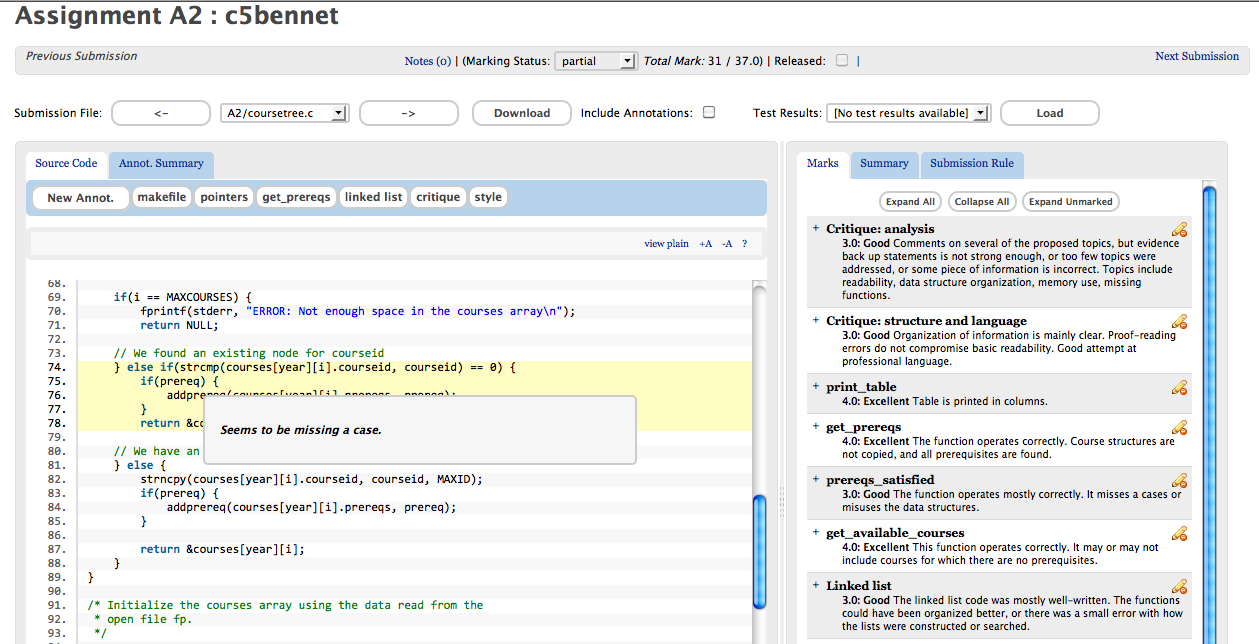
\includegraphics[width=\textwidth]{images/graderview.png}
  }
      %  
    \caption{Grader's view}
  \end{center}
\end{figure}
\end{block}
}

\frame{
  \frametitle{MarkUs' features}

  \begin{block}{Pedagogical improvement (teachers)}  
    	\begin{itemize}
    	\item Follow the \textbf{marking scheme} to grade the papers
	\item Use existing annotations (source code, images and PDF) or create new ones 
	\item Multiple graders for the same paper 
  	\end{itemize}
	\vspace{-1em}
\begin{figure}
  \begin{center}
  \scalebox{0.29}{
    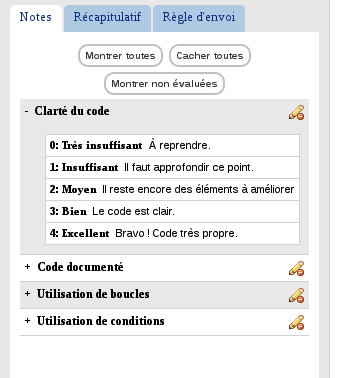
\includegraphics[width=\textwidth]{images/markus-criteres.png}
  }
      %  
    \caption{Criteria definition}
  \end{center}
\end{figure}
\end{block}
}

\frame{
  \frametitle{MarkUs' features}

  \begin{block}{Pedagogical improvement (teachers)}  
    	\begin{itemize}
	\item Management of multiple assignements in the context of one MarkUs instance per course
	\item Automatic management of \textbf{deadlines} with configurable penalties for late submission
    	\item Possibility to view and grade a \textbf{previous} version of the work 
  	\end{itemize}
\end{block}
}

\frame{
  \frametitle{MarkUs' features}

  \begin{block}{Pedagogical improvement (student)}  
    	\begin{itemize}
	\item Group creation \textbf{depending on the assignment}
    	\item Comments and annotations export
	\item Improved and faster feedback
	\item Comments can be checked on-line \textbf{anytime} \textbf{anywhere}
  	\end{itemize}
	\vspace{-1em}
\begin{figure}
  \begin{center}
  \scalebox{0.55}{
    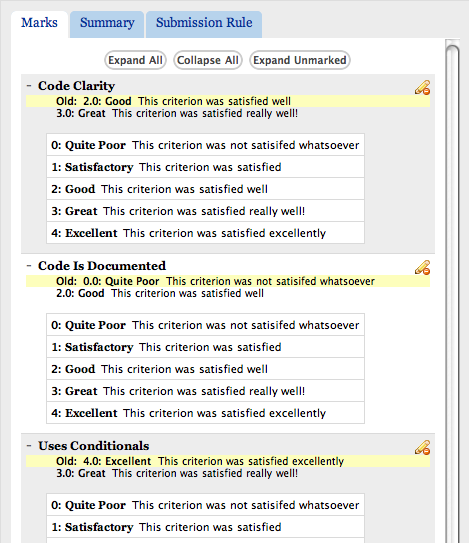
\includegraphics[width=\textwidth]{images/Doc_Admin_Remarking.png}
  }
      %  
    \caption{Results' page as shown to students}
  \end{center}
\end{figure}
\end{block}
}

\subsection*{Demo}

\frame{
  \frametitle{Demo}
Let us give you a short demo of the software…
}

\frame
{
  \frametitle{MarkUs: key figures}

\begin{block}{MarkUs, a free software to assess students' works}
\begin{itemize}
\item ECN: 
\begin{itemize}
\item Two CS courses of the common engineering core every year + CS major 
\item \textbf{750 students impacted} every year
\item Up to 350 students per course
\end{itemize}
\item UoT: 
\begin{itemize}
\item 8 different courses in CS and Engineering
\item A total of 1200 students impacted 
\item Up to \textbf{650 students} per course 
\end{itemize}
\item UoW: 
\begin{itemize}
\item Two large courses every term 
\item More than \textbf{800 students impacted} every term
\end{itemize}
\item Since 2008: contribution of \textbf{more than 45 undergraduate students} 
\end{itemize}
\end{block}
}

\section*{Impact of MarkUs on the teaching and learning processes}

% Cette partie pour donner un aperçu des fonctionnalités de MarkUs et leur impact sur l'enseignement

\subsection*{Benefits for teachers}

\frame{
  \frametitle{Why teachers enjoy MarkUs:}
\begin{itemize}
\item Management of a \textbf{large number} of submissions (previous experiments went up to 900 students)
\item \textbf{Centralized} and \textbf{versioned} submission of the papers 
\item \textbf{Decrease of the time} required for grading the papers: between 14\% and 50\%
\item \textbf{Decrease of the number of late submissions}: drop from 15-20\% to 5-10\%
\item \textbf{Dematerialization} 
\item Supports \textbf{nomadism}
\end{itemize}
}

\subsection*{Benefits for students}

\frame{
  \frametitle{Why students enjoy MarkUs}
\begin{itemize}
\item A \textbf{unique} tool for submitting and getting the assessment results
\item Improvement of the \textbf{delay} to get the assessment results 
\item \textbf{Decrease of the number of papers} whose results and feedback are given after the final exam
\item \textbf{Permanent} access to previous works annotated by teachers 
\end{itemize}
}

\subsection*{Benefits for teaching and learning}

\frame{
  \frametitle{MarkUs' beneficial effects}
   \begin{block}{Impact on the teaching activy:}
  	\begin{itemize}
	\item Improved \textbf{logistic} management 
	\item \textbf{Unification} of marking criteria
	\item Grading becomes quite \textbf{fun}
  	\end{itemize} 
  \end{block}
}


\frame{
  \frametitle{MarkUs' beneficial effects}
  \begin{block}{Impact on the learning process:}
  	\begin{itemize}
    	\item Better respect of \textbf{deadlines} by students
	\item Every \textbf{student} gets access to the feedback given on his work 
	\item \textbf{More interest} in the comments and annotations left by teachers
	\item \textbf{Prompt feedback} allows to take comments into account for preparing the next assignments.
  	\end{itemize} 
  \end{block}
}

\section*{Summary and further work}

\frame
{
  \frametitle{Conclusion}

\begin{alertblock}{Aim}
How to improve and streamline the grading workflow? 
\end{alertblock}

\begin{block}{MarkUs}

\begin{itemize}
\item \textbf{Free} software 
\item Annotation of \textbf{source code}, \textbf{.PDF} and \textbf{images} 
\item Easy to handle
\item Costs only the time necessary to install and maintain the running instances
\item Towards the creation of \textbf{virtuous circles} : users $\rightarrow$ contributors $\rightarrow$ mentors
\end{itemize}
\end{block}
}

\subsection*{Further work}

\frame{
  \frametitle{Improvements to come}
  
  \begin{block}{Widen the use of MarkUs}
  	\begin{itemize}
	\item Incorporate an \textbf{automatic testing framework}
	\item Integrate a \textbf{plagiarism detection tool} into the application
	\item Extend the use of MarkUs to meet the needs of \textbf{research peer-reviewing} processes
	\end{itemize}
\end{block}
}

\subsection*{References}

\frame{
  \frametitle{More info}
  
\begin{block}{Links and contacts}
\begin{itemize}
\item Project website: \url{http://markusproject.org}
\item Try the software on-line: \url{http://markusproject.org/admin-demo}
\item Source: \url{https://github.com/MarkUsProject/Markus}
\item EAT-TICE Ecole Centrale de Nantes website: \url{http://eat-tice.ec-nantes.fr}
\item IRC channel: \#markus and \#markus-fr on irc.freenode.net
\item Mailing list : \url{markus-dev@cs.toronto.edu}
\end{itemize}
\end{block}
}


%\bibliography{biblio}
%\bibliographystyle{alpha}

\end{document}
